\documentclass[a4paper, 12pt]{article}
\usepackage[a4paper,top=1.5cm, bottom=1.5cm, left=1cm, right=1cm]{geometry}

% Работа с русским языком
\usepackage[utf8]{inputenc}
\usepackage{mathtext}                % русские буквы в формулах
\usepackage[english, russian]{babel} % локализация и переносы

\usepackage{graphicx}   % Вставка изображений
\usepackage{float}      % "Плавающие" изображения3
\usepackage{wrapfig}    % Обтекание фигур (таблиц, картинок и прочего)
\usepackage{subfig}
\graphicspath{ {./images/} }

\usepackage{tabularx}
\usepackage{multirow}
\usepackage{booktabs}
\usepackage{amsmath}
\usepackage{amsfonts}
\usepackage{indentfirst}
\usepackage{longtable}
\usepackage{natbib}
\usepackage{bm}

\newcommand{\angstrom}{\text{\normalfont\AA}}
\newcommand{\e}[1]{\text{$\cdot10^{#1}$}}
\newcommand{\m}{\; м}
\newcommand{\mm}{\; мм}
\newcommand{\um}{\; мкм}
\newcommand{\A}{\; А}
\newcommand{\V}{\; В}
\newcommand{\uV}{\; мкВ}
\newcommand{\cels}{\; ^\circ С}

%%% Колонтитулы
\usepackage{titleps}
\newpagestyle{main}{
	\setheadrule{0.4pt}
	\sethead{Отчёт о выполнении лабораторной работы 1.3}{}{}
	\setfootrule{0.4pt}                       
	\setfoot{ФРКТ МФТИ, 2024}{}{\thepage} 
}
\pagestyle{main}  

\begin{document}
    \begin{titlepage}
	\begin{center}
            {\large МОСКОВСКИЙ ФИЗИКО-ТЕХНИЧЕСКИЙ ИНСТИТУТ (НАЦИОНАЛЬНЫЙ ИССЛЕДОВАТЕЛЬСКИЙ УНИВЕРСИТЕТ)}
	\end{center}
 
	\begin{center}
		{\large Физтех-школа радиотехники и компьютерных технологий}
	\end{center}
	
	\vspace{8cm}
	{\LARGE
		\begin{center}
                {\bf Отчёт о выполнении лабораторной работы 1.3}\\
                Эффект Рамзауэра
		\end{center}
	}
	\vspace{3 cm}
	\begin{flushright}
		{\Large Авторы: \\ 
        Тихонов Дмитрий Романович, \\ студент группы Б01-206а \\
        Павловский Кирилл Михайлович, \\ студент группы Б01-206а}
	\end{flushright}
	\vspace{4cm}
	\begin{center}
		\Large Долгопрудный, 2024
	\end{center}
    \end{titlepage}


    \section{Введение}

    \noindent \textbf{Цель работы:} исследовать энергетические зависимости вероятности рассеяния электронов атомами инертного газа; определить энергии электронов, при которых наблюдается \textit{просветление} инертного газа; оценить размер внешней электронной оболочки инертного газа. \\
	
    \noindent \textbf{В работе используются:} тиратрон ТГ3-01/1.3Б, вольтметры GDM-8145, блок источников питания, осциллограф GOS-620.
    
    \section{Теоретическое введение}

    Карл Рамзауэр исследовал зависимость поперечных сечений упругого рассеяния электронов (с энергией до 10 эВ) на атомах аргона. В результате этих исследований было обнаружено явление, получившее название \textit{эффекта Рамзауэра}.
	
    С точки зрения квантовой теории атом по отношению к электронной волне ведет себя как преломляющая среда с относительным показателем преломления
    
    \begin{equation}
        n = \frac{\lambda}{\lambda^\prime} = \sqrt{1-\frac{U}{E}},
    \end{equation}
    
    где $U$, $E$ -- потенциальная и полная энергии электрона внутри атома соответственно.
	
    Будем считать, что электрон рассеивается на одномерной прямоугольной потенциальной яме конечной глубины. Такая модель является хорошим приближением для атомов тяжелых инертных газов, отличающихся наиболее компактной структурой и резкой внешней границей. Решение задачи о прохождении частицы с энергией $E$ над потенциальной ямой шириной $l$ и глубиной $U_0$ не составит труда найти из уравнения Шредингера:
    
    \begin{equation}
        \psi^{\prime\prime} + k^2\psi = 0, \ \text{где}\
        k^2 = \begin{cases}
            2mE/\hbar^2, & x < 0, \ x  >l; \\
            (2mE+U_0)/\hbar^2, & 0 < x < l.
        \end{cases}
    \end{equation}
    
    Коэффициент прохождения равен отношению квадратов амплитуд прошедшей и падающей волн и определяется выражением:
    
    \begin{equation}
        \frac{1}{D} = 1 + \frac{U_0^2}{4E(E+U_0)}\sin^2(k_2l).
    \end{equation}
    
    Минимум последнего выражения отвечает квантовому аналогу просветления оптики, так как при выполнении условия
	\begin{equation}
		\label{eq:condition}
		\sqrt{\frac{2m(E+U_0)}{\hbar^2}}l = \pi n, \ n = 1, 2, 3 \dots
	\end{equation}
	
    коэффициент прохождения частицы над ямой становится равным единице, то есть достигает своего максимального значения.
    
    Отметим, что условие (\ref{eq:condition}) легко получить, рассматривая интерференцию электронов волн де Бройля в атоме:
    
    \begin{itemize}
        \item Условие первого интерференционного максимума:
            \begin{equation}
                \label{eq:condition_max}
                2l = \frac{h}{\sqrt{2m (E_1 + U_0)}}.
            \end{equation}
        \item Условие первого интерференционного минимума:
            \begin{equation}
                \label{eq:condition_min}
                2l =\frac{3}{2} \frac{h}{\sqrt{2m (E_2 + U_0)}}.
            \end{equation}			
    \end{itemize}

    Решая совместно уравнения (\ref{eq:condition_max}) и (\ref{eq:condition_min}), получим
	
    \begin{equation}
        \label{eq:l}
	l = \frac{h\sqrt{5}}{\sqrt{32m(E_2-E_1)}}.
    \end{equation}
	
    Понятно, что энергии $E_1$ и $E_2$ соответствуют энергиям электронов, прошедших разность потенциалов $V_1$ и $V_2$, т.е. $E_1 = eV_1$ и $E_2 = eV_2$. 
	
    По измеренным величинам $E_1$ и $E_2$, используя формулы (\ref{eq:condition_max}, \ref{eq:condition_min}), можно рассчитать эффективную глубину потенциальной ямы атома:
	
    \begin{equation}
        \label{eq:U_0}
        U_0 = \frac{4}{5}E_2 - \frac{9}{5}E_1
    \end{equation}
    
    \newpage
    
    \section{Методика измерений и экспериментальная установка}

    \subsection{Описание экспериментальной установки}

    \begin{figure}[H]
        \centering
        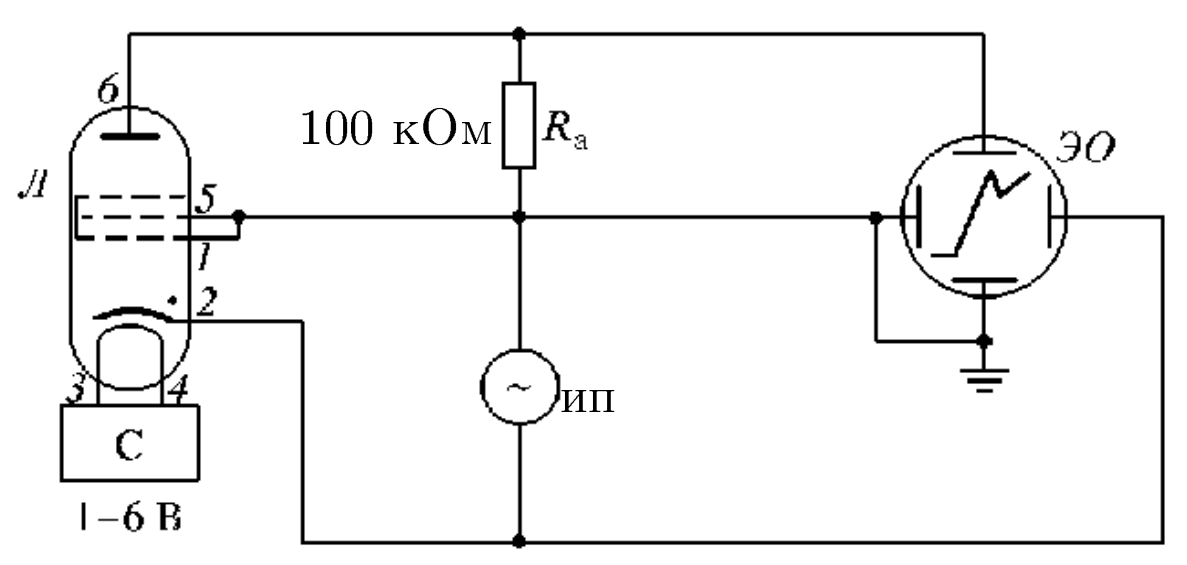
\includegraphics[width = 0.3\textwidth]{images/schm1.png}
        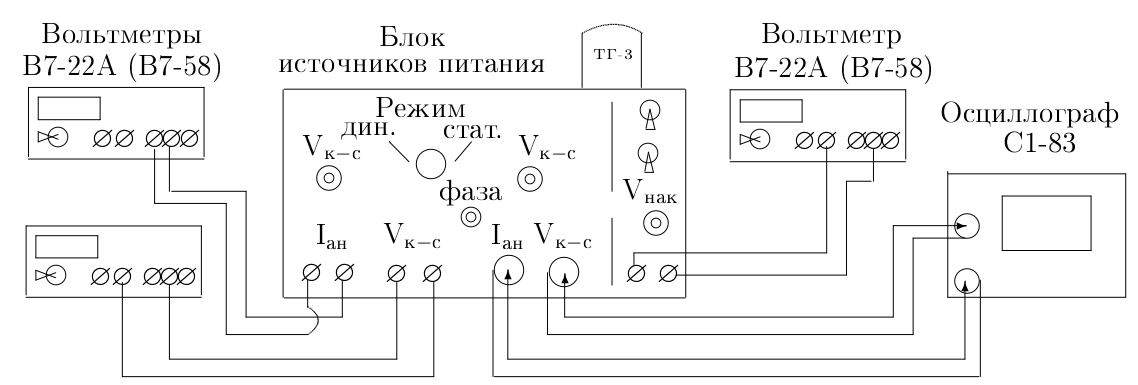
\includegraphics[width = 0.6\textwidth]{images/schm2.png}
        \caption{Схема подключения тиратрона (слева) и блок-схема экспериментальной установки (справа)}
        \label{img:exp_scheme}
    \end{figure}

    \begin{wrapfigure}{r}{0.3\textwidth}
        \centering
        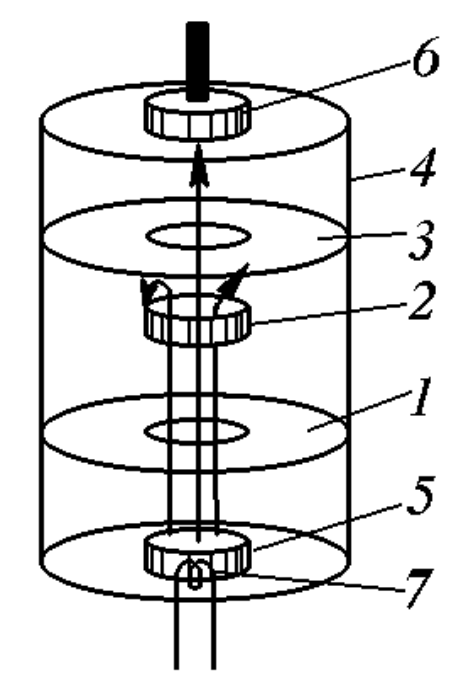
\includegraphics[width = 0.15\textwidth]{images/tiratron.png}
        \caption{Схема тиратрона: 1, 2, 3 -- сетки с одинаковым потенциалом, 4 -- внешний металлический цилиндр, 5 -- катод, 6 -- анод, 7 -- накаливаемая спираль.}
        \label{img:tiratron}
    \end{wrapfigure}

    В работе для наблюдения эффекта Рамзауэра используется тиратрон ТГ3-01/1.3Б, заполненный инертным газом (рис. \ref{img:tiratron}). Электроны, эмитируемые катодом тиратрона, ускоряются напряжением $V$, приложенным между катодом и ближайшей к нему сеткой. Затем электроны рассеиваются на атомах инертного газа. Рассеянные электроны отклоняются в сторону и уходят на сетку, а оставшаяся часть электронов достигает анода и создаёт анодный ток $I_а$.

    Схема экспериментальной установки приведена на рисунке \ref{img:exp_scheme}. Лампа тиратрона расположена на корпусе блок источников питания. Напряжение к электродам лампы подаётся от источников питания, находящихся в корпусе прибора. Регулировка напряжения и выбор режима работы установки производится при помощи ручек управления, выведенных на лицевую панель блока источников питания.

    \subsection{Оборудование и приборы}

    \begin{itemize}
        \item Тиратрон ТГ3-01/1.3Б.
                    
        \item Вольтметры GDM-8145. Все вольтметры измеряют в пределе 20 В. Погрешность измерения $\sigma = \pm (0.03\% \; rdg + 4 \; digits)$.
		
        \item Блок источников питания.
		
        \item Осциллограф GOS-620. 
    \end{itemize}

    \subsection{Методика эксперимента}

    Электроны эмитируются катодом, ускоряются напряжением $V$ и рассеиваются на атомах газа. Сетки соединены между собой и имеют один потенциал, примерно равный потенциалу анода. Рассеянные электроны отклоняются и уходят на сетку, а оставшиеся достигают анода, создавая ток $I_\text{a}$. Таким образом, поток электронов на расстоянии $x$ от ускоряющей сетки уменьшается с ростом $x$. Реальная вольт-амперная характеристика тиратрона описывается соотношением
    
    \begin{equation}
        \label{eq:VAC}
        I_\text{a} = I_0 e^{- C w(V)}, \qquad C = L n_\text{а} \Delta_{а},
    \end{equation}
    
    где $I_0 = eN_0$ -- ток катода, $I_\text{a} = eN_a$ -- анодный ток, $L$ --  расстояние между катодом и анодом, $\Delta_\text{a}$ -- площадь поперечного сечения атома, $n_\text{a}$ -- концентрация газа в лампе, $w(V)$ -- вероятность рассеяния на атоме.
    
    Формулу \eqref{eq:VAC} можно переписать в виде
    \begin{equation}
        \label{eq:w(V)}
        w(V) = -\dfrac{1}{C}\ln \dfrac{I_\text{a}(V)}{I_0}.
    \end{equation}

    \newpage
	
    \section{Результаты измерений и обработка данных}
    
    \subsection{Динамический режим}

    \begin{table}[H]
        \centering
        \begin{tabular}{ccccccccc}
            \toprule
            $V_{\text{накал}}, \V$ & $V_{\text{мин}}, \V$ & $\sigma_{V_{\text{мин}}}, \V$ & $V_{\text{макс}}, \V$ & $\sigma_{V_{\text{макс}}}, \V$ & $U_{\text{пробой}}, \V$ & $\sigma_{U_{\text{пробой}}}, \V$ \\ \midrule
            2.51 & 6.8 & 0.4 & 2.1 & 0.3 & 13.1 & 0.6 \\
            2.77 & 7.1 & 0.4 & 2.2 & 0.3 & 12.3 & 0.6 \\
            2.97 & 6.5 & 0.4 & 2.0 & 0.3 & 11.0 & 0.5 \\
            \toprule
        \end{tabular}
        \caption{Результаты измерений в динамическом режиме}
        \label{table:dynamic}
    \end{table}

    По результатам измерения в динамическом режиме (табл. \ref{table:dynamic}) определим эффективный размер (диаметр) электронной оболочки атома инертного газа
    $$
    l = \frac{h\sqrt{5}}{\sqrt{32 m_e e (V_{мин} - V_{макс})}}
    $$
    
    и эффективную глубину потенциальной ямы атома
    $$
    U_0 = e \left(\frac{4}{5} V_{мин} - \frac{9}{5} V_{макс} \right).
    $$
    
    Оценим погрешность $l$ по формуле косвенных измерений:
    $$
    \sigma_l = \frac{1}{2} l \cdot \frac{\sqrt{\sigma_{V_{мин}}^2 + \sigma_{V_{макс}}^2}}{V_{мин} - V_{макс}}.
    $$
	
    Оценим погрешность $U_0$ по формуле косвенных измерений:
    $$
    \sigma_{U_0} = \sqrt{\left(\frac{4}{5} \sigma_{V_{мин}}\right)^2 + \left(\frac{9}{5} \sigma_{V_{макс}}\right)^2}.
    $$
    	
    При измерении напряжения осциллографом существует ошибка, связанная с наличием контактной разности потенциалов, оценить которую напрямую не удаётся. С другой стороны, при вычислении эффективного размера электронной оболочки атома $l$ используются значения напряжение не по отдельности, а их разность. В предположении, что контактная разность потенциалов не зависит от значения измеряемого напряжения, при вычислении $l$ контактная разность потенциалов не влияет на итоговый результат, тем не менее она вносит дополнительную ошибку при нахождении эффективной глубины потенциальной ямы атома $U_0$. Результаты вычислений приведены в таблице \ref{table:atom}.
	
    \begin{table}[H]
    \centering
    \begin{tabular}{c c c c c c }
        \toprule
        $V_{\text{накал}}, \V$ & $l, \angstrom$ & $\sigma_l, \angstrom$ & $U_0, \text{эВ}$ & $\sigma_{U_0}, \text{эВ}$ \\ \midrule
        2.51 & 3.2 & 0.2 & 1.7 & 0.6 \\
        2.77 & 3.1 & 0.2 & 1.7 & 0.6 \\
        2.97 & 3.2 & 0.2 & 1.6 & 0.6 \\ 
        \toprule
    \end{tabular}
    \caption{Динамический режим. Эффективный размер электронной оболочки атома $l$ и эффективная глубина потенциальной ямы атома $U_0$.}
    \label{table:atom}
    \end{table}

    Геометрические размеры тиратрона таковы, что ионизационный потенциал практически совпадает с напряжением пробоя. Среднее значение напряжения пробоя: \\
    $$
    U_\text{пробой} = 12 \V.
    $$
    
    Погрешность определяется по формуле
    $$
    \sigma_{U_{пробой}} = \sqrt{\sigma_{приб}^2 + \sigma_{случ}^2} = 1.1 \V
    $$
    
    $$
    \sigma_{случ} = \sqrt{\frac{1}{N - 2}\sum_i \frac{\left(U_i - \overline{U}\right)^2}{N}} = 0.9 \V
    $$
	
    Приборную погрешность измерения среднего напряжения оценим как среднюю погрешность отдельных измерений $\sigma_{приб} = 0.6 \V$.
	
    Итого, ионизационный потенциал
    $$
    U_{ион} = \left( 12 \pm 1 \right) \; эВ,
    $$
    
    что совпадает с ионизационным потенциалом ксенона $U_{ион}^{Xe} = 12.1 \; эВ$.

    \subsection{Статический режим}

    Построим графики зависимости $I_{анод}(V_{катод})$ при разных напряжениях накала тиратрона.

    \begin{figure}[H]
        \centering
        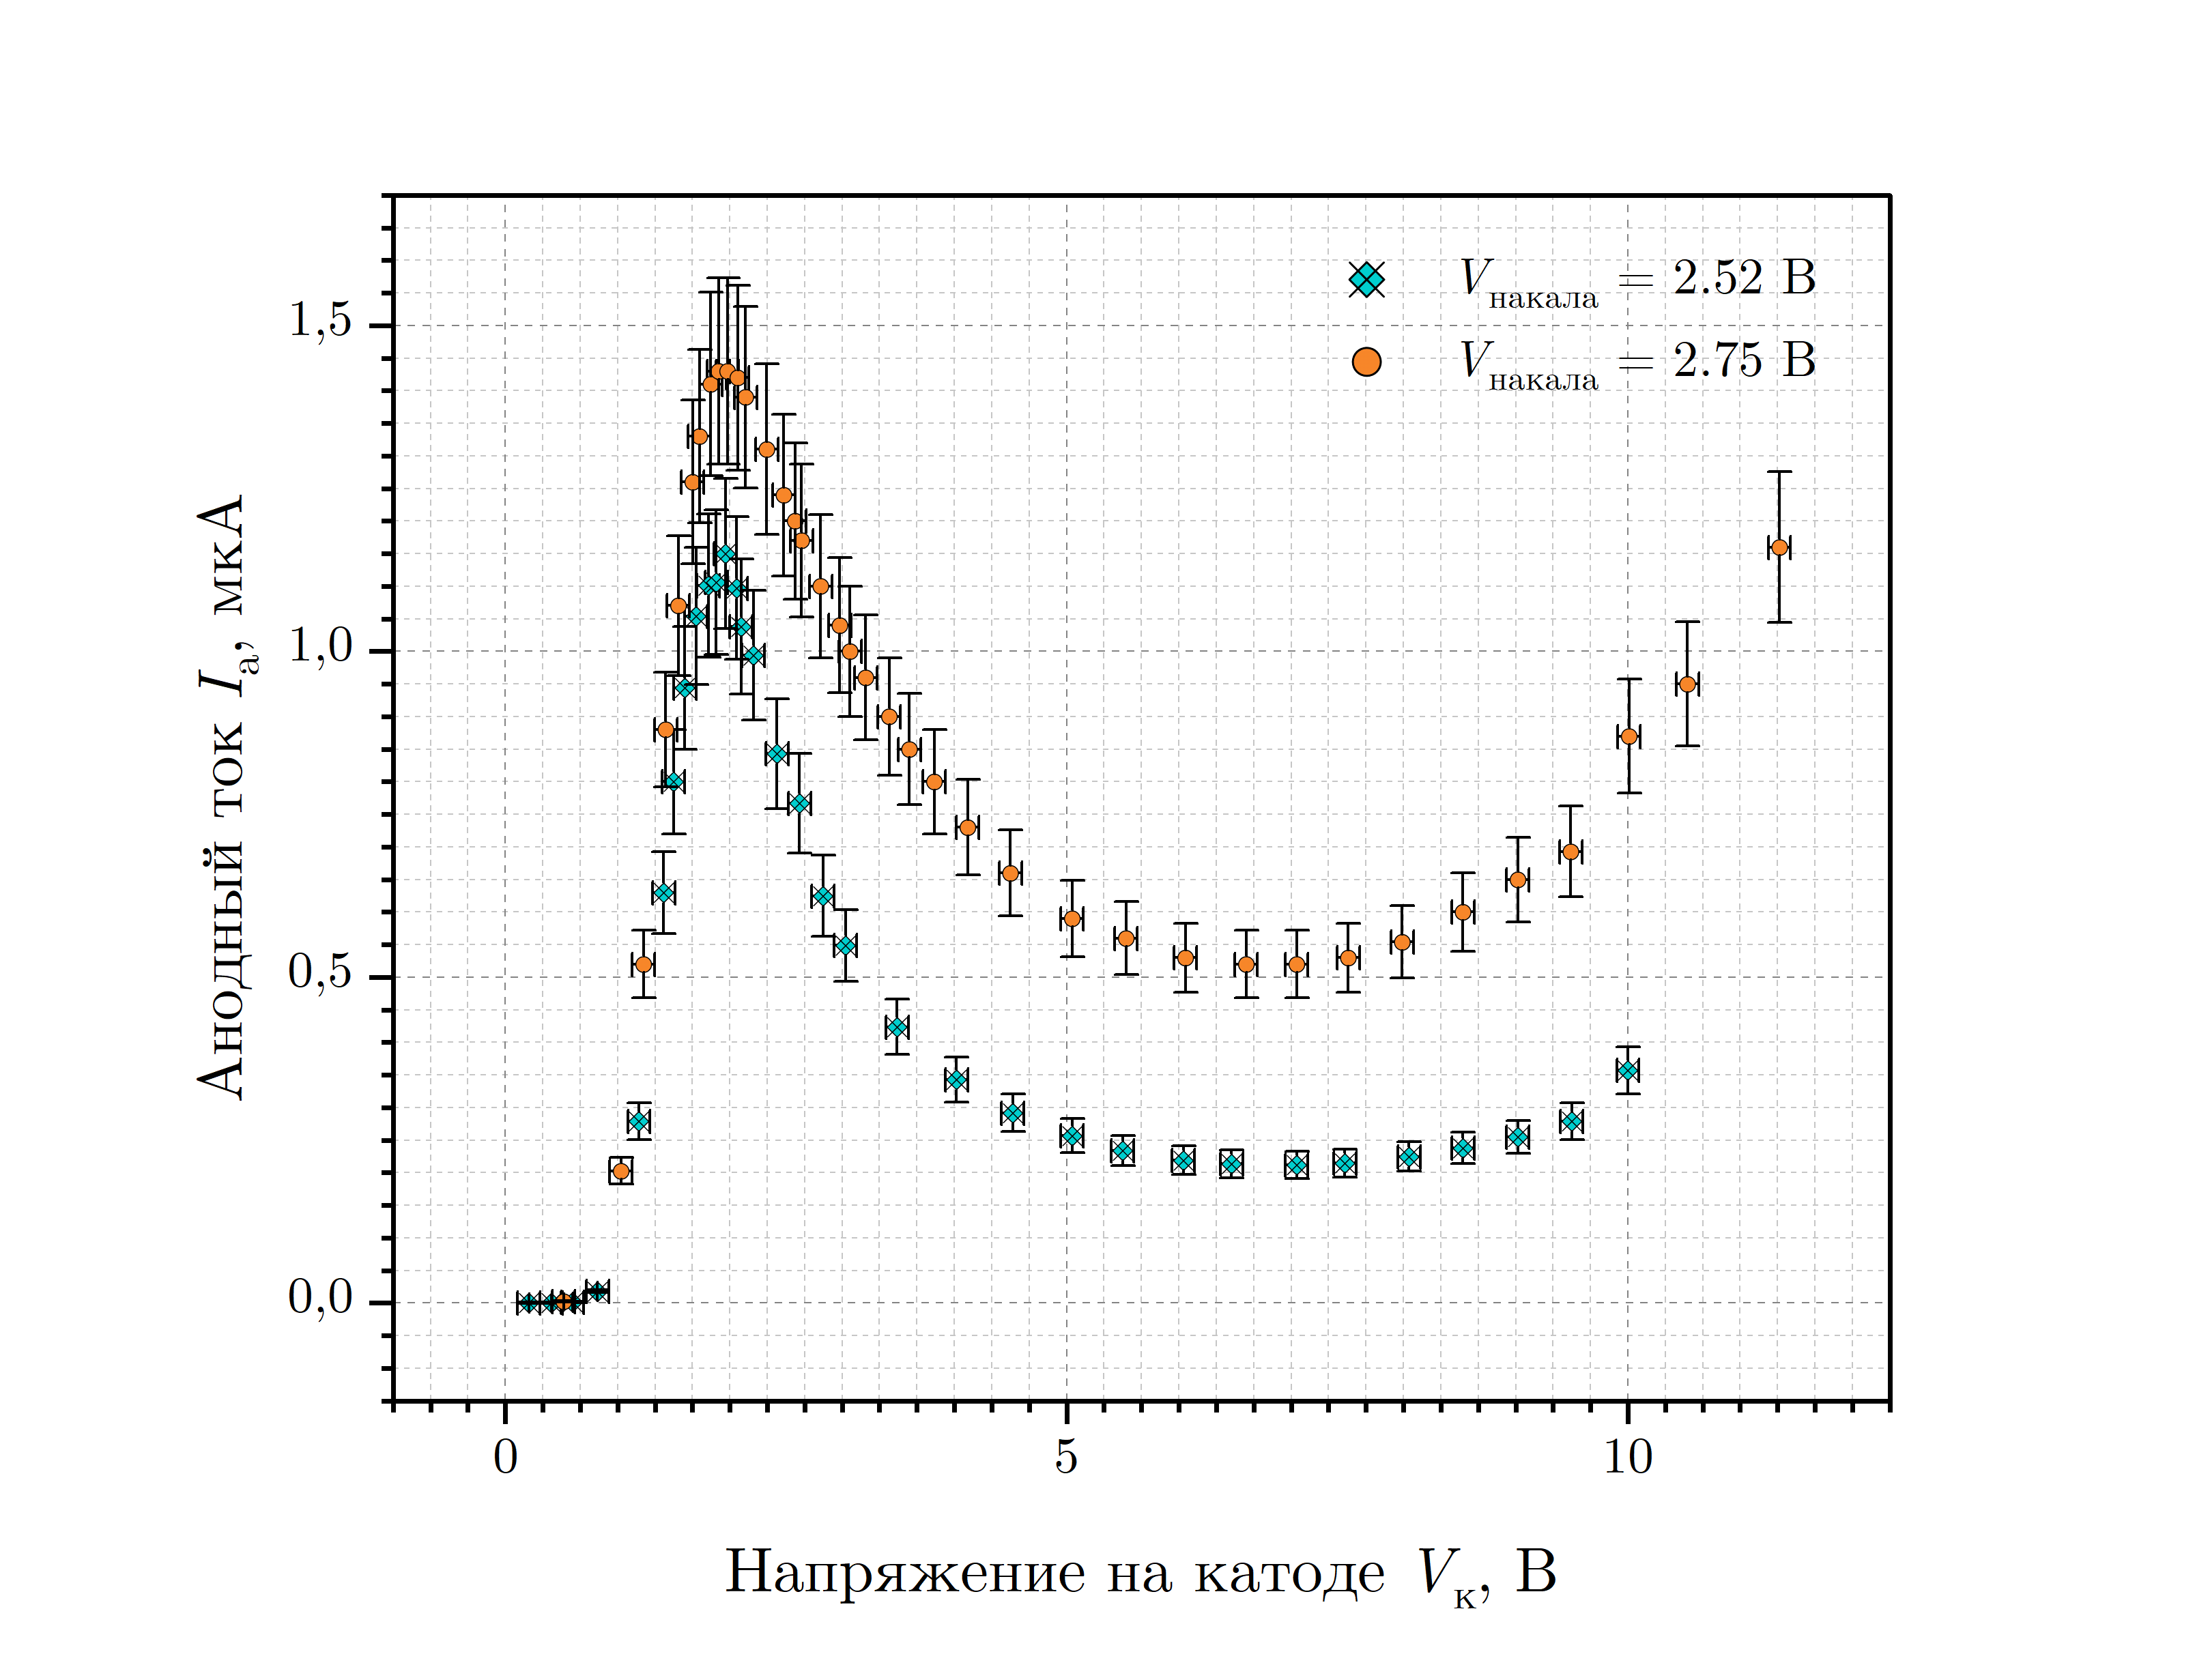
\includegraphics[width = 0.7\textwidth]{images/graph_VAC.png}
        \caption{График зависимости тока анода $I_{анод}$ от напряжения катода $V_{катод}$}
    \end{figure}
	
    По графику $I_{анод}(V_{катод})$ определим напряжения максимумов и минимумов.
	
    \begin{table}[H]
        \centering
        \begin{tabular}{c c c c c c }
            \toprule
            $V_{\text{накал}}, \V$ & $V_{min}, \V$ & $\sigma_{V_{min}}, \V$ & $V_{max}, \V$ & $\sigma_{V_{max}}, \V$ \\ \midrule
            2.51 & 3.2 & 0.2 & 1.7 & 0.6 \\
            2.77 & 3.1 & 0.2 & 1.7 & 0.6 \\
            2.97 & 3.2 & 0.2 & 1.6 & 0.6 \\ 
            \toprule
        \end{tabular}
        \caption{Статический режим. Напряжения максимумов и минимумов на графике $I_{анод}(V_{катод})$}
        \label{table:st}
    \end{table}

    Определим эффективный размер электронной оболочки атома $l$ и эффективная глубину потенциальной ямы атома $U_0$.
	
    \begin{table}[H]
        \centering
        \begin{tabular}{c c c c c c }
            \toprule
            $V_{\text{накал}}, \V$ & $l, \angstrom$ & $\sigma_l, \angstrom$ & $U_0, \text{эВ}$ & $\sigma_{U_0}, \text{эВ}$ \\ \midrule
            2.52 & 3.04 & 0.01 & 2.11 & 0.04 \\
            2.75 & 3.17 & 0.01 & 1.86 & 0.04 \\
            \toprule
        \end{tabular}
        \caption{Статический режим. Эффективный размер электронной оболочки атома $l$ и эффективная глубина потенциальной ямы атома $U_0$.}
        \label{table:atom-st}
    \end{table}

    Построим график зависимости вероятности рассеяния электронов (с точностью до константы) от энергии:
    $$
    w(V) = -\frac{1}{C} \ln{\frac{I_{анод}(V)}{I_0}}
    $$
    
    \begin{figure}[H]
        \centering
        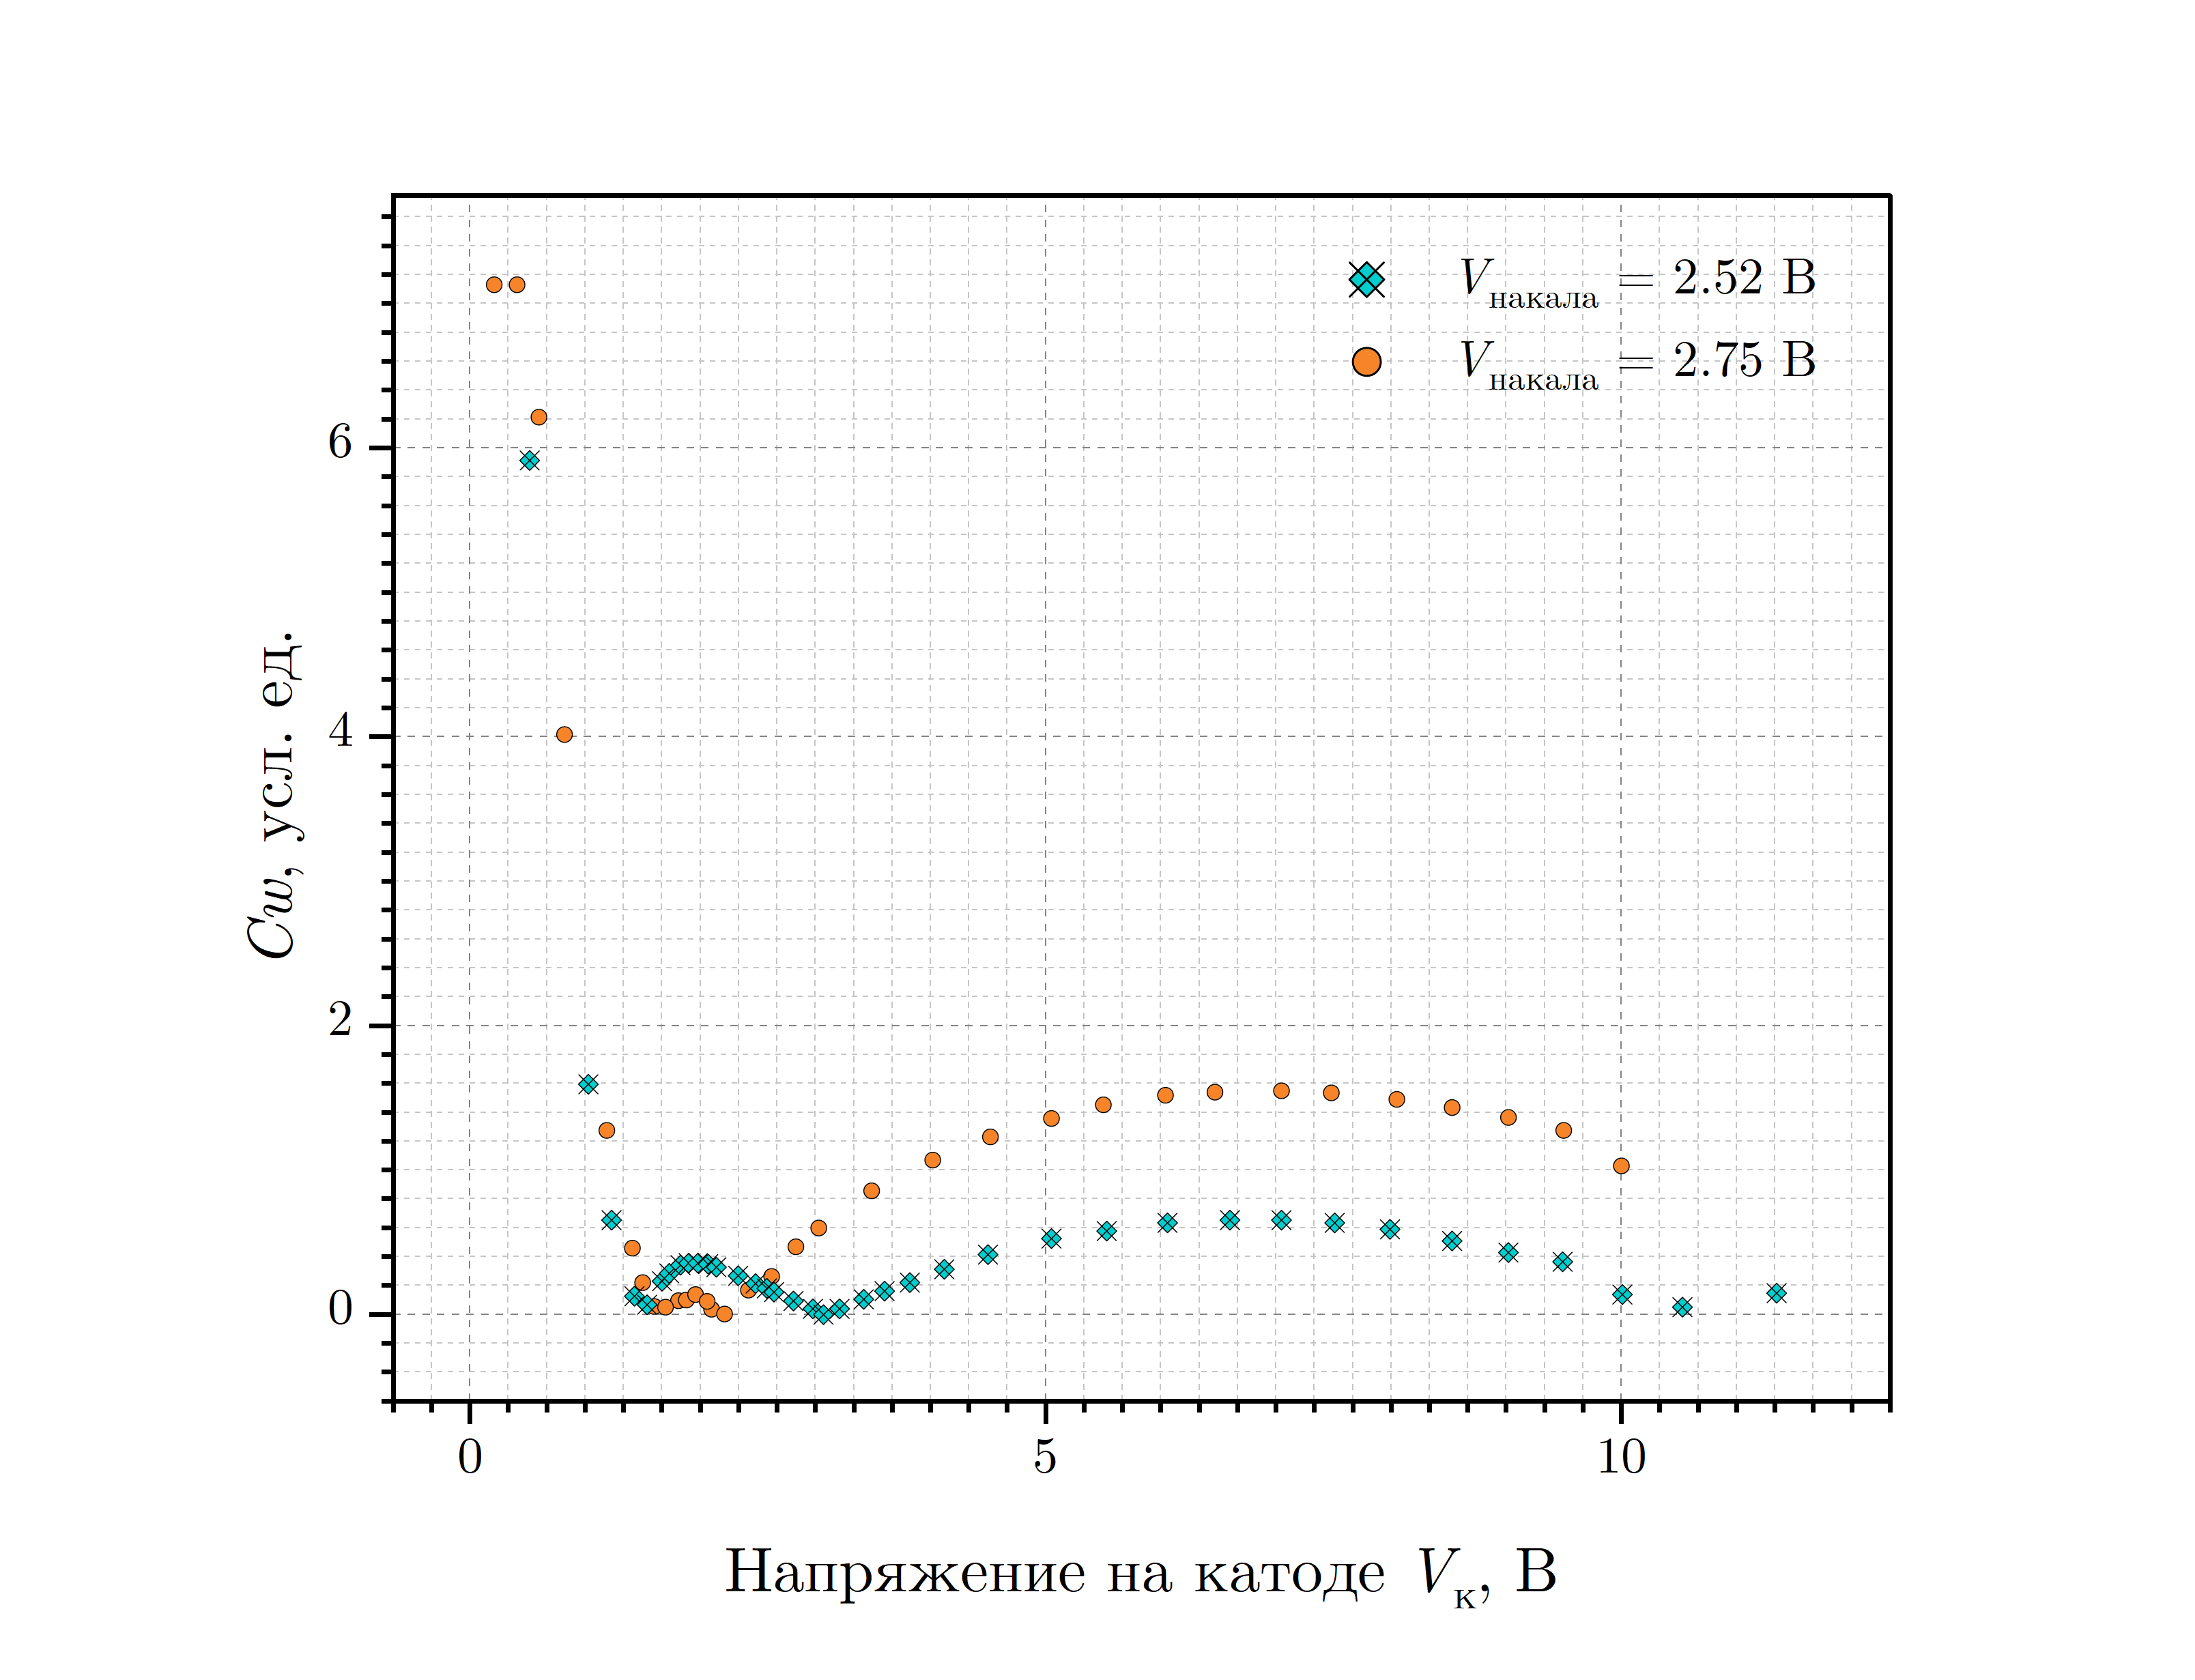
\includegraphics[width = 0.7\textwidth]{images/graph_w(V).png}
        \caption{График зависимости вероятности в условных единицах от напряжения катод-сетка $V_{катод}$}
    \end{figure}
    
    \section{Заключение}
    
    \begin{itemize}
       \item В работе были оценены эффективные размеры электронной оболочки атома инертного газа и эффективная глубина потенциальной ямы статическим и динамическим методами.
        \item С помощью динамического метода был определён ионизационный потенциал инертного газа:
        $$
        U_{ион} = \left( 12 \pm 1 \right) \; эВ
        $$
        что совпадает с ионизационным потенциалом ксенона $U_{ион}^{Xe} = 12.1 \; эВ$, поэтому можно предположить, что в тиратроне находится ксенон.
    \end{itemize}
    
\end{document}